\subsection{BlockCerts}
Se define a si mismo 
como un estándar abierto   desarrollado por el MIT Media Lab y Learning Machine, para la construcción  de  aplicaciones que emiten y verifican registros oficiales basados
en la Blockchain. Pueden incluir certificados de registros civiles, académicos, licencias profesionales y más. 
Consiste en una librería con herramientas y apps móviles habilitando un ecosistema descentralizado, basado en estándar y habilitando verificación sin necesidad de la confianza mediante la tecnología  Blockchain \cite[]{blockcerts_introduction_nodate}.
Algunas universidades como el Instituto Tecnológico de Massachusetts (MIT), Tecnológico de Monterrey, la Universidad Harvard, la Universidad de California en Berkeley lo aplican. El 
estándar plantea que los certificados puedan ser compatibles a un nivel global, sin importar
la  Blockchain que se utilice pudiendo ser Bitcoin, Ethereum u otra \cite[]{edublocs_nueve_2019,criptomonedas_tv_entrevista_2018}. 

\begin{figure}[H]
  \centering
  {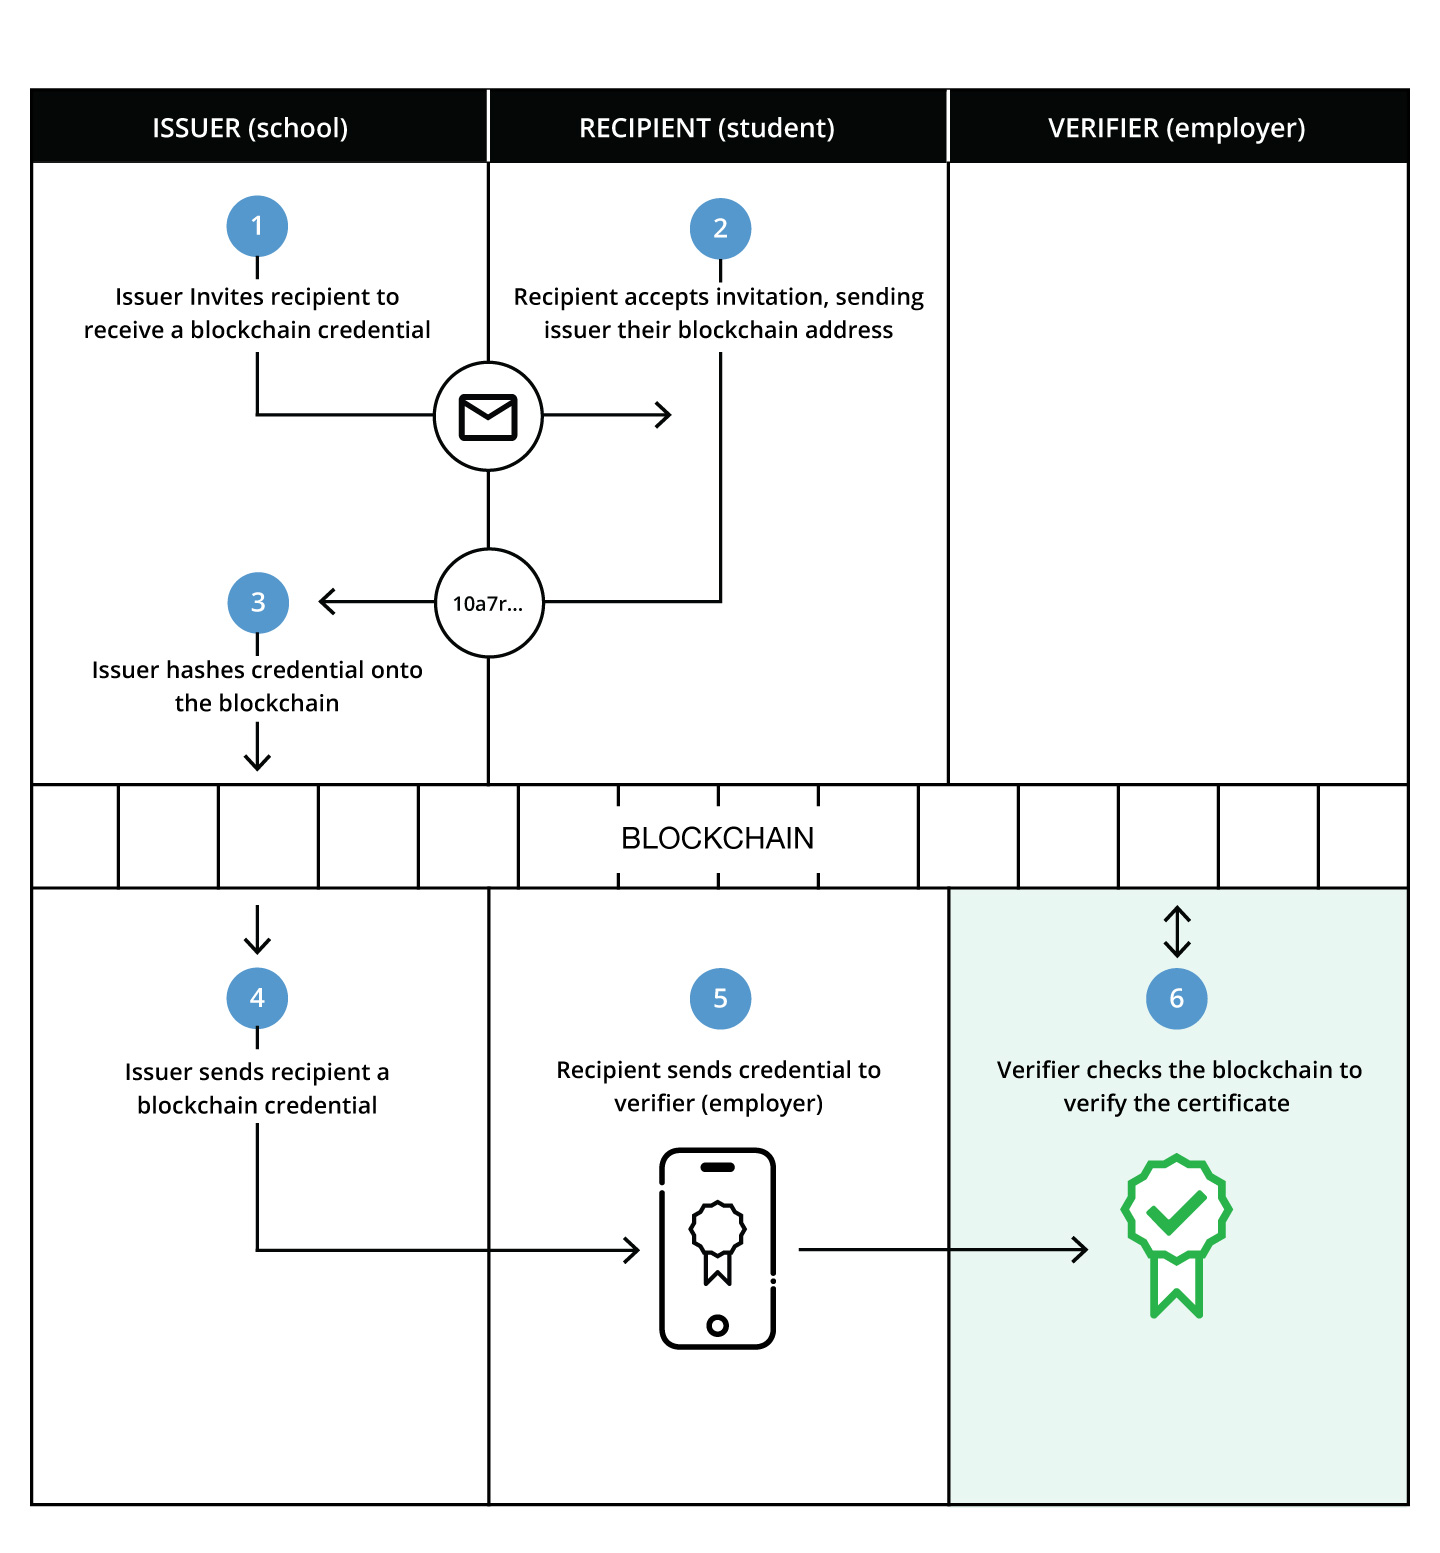
\includegraphics[scale=0.3]{blockcerts_how_it_works.jpg}}
  \caption{Imagen extraída de la página oficial de BlockCerts}
  \label{img:blockcerts_how_it_works}
\end{figure}

El flujo básico que se visualiza en  la figura \ref{img:blockcerts_how_it_works}   para comprobar que
un certificado se encuentra almacenado en la  Blockchain y es validado por un instituto se explica a continuación:

En el paso 1, el emisor o institución invita a un usuario a que brinde su dirección de cuenta o su clave pública creada 
descargando, la aplicación movil que provee BlockCerts. En el paso 2, el usuario envía al emisor su clave pública.
El paso 3 y 4, el emisor crea el hash a partir del certificado y lo almacena en la  Blockchain para luego enviar un archivo de tipo JSON 
\footnote{JavaScript Object Notation es un formato basado en texto estándar para representar datos estructurados \cite[]{mozilla_trabajando_json}.}, que contiene
la información sobre el documento del estudiante o dueño del certificado. En el paso 5, puede enviar este documento a cualquier empresa o individuo que desee.
 En el paso 6 el usuario que posee el archivo puede verificarlo en el sitio web de  BlockCerts \cite[]{blockcerts_introduction_nodate}.

 